%%%%%%%%%%%%%%%%%%%% book.tex %%%%%%%%%%%%%%%%%%%%%%%%%%%%%
%
% sample root file for the chapters of your "monograph"
%
% Use this file as a template for your own input.
%
%%%%%%%%%%%%%%%% Springer-Verlag %%%%%%%%%%%%%%%%%%%%%%%%%%


% RECOMMENDED %%%%%%%%%%%%%%%%%%%%%%%%%%%%%%%%%%%%%%%%%%%%%%%%%%%
\documentclass[pdftex,12pt, oneside]{article}

% choose options for [] as required from the list
% in the Reference Guide, Sect. 2.2
%\usepackage[paperwidth=8.5in, paperheight=13in]{geometry} % Folio
\usepackage[paperwidth=8.27in, paperheight=11.69in]{geometry} % A4

\usepackage{makeidx}         % allows index generation
\usepackage{graphicx}        % standard LaTeX graphics tool
                             % when including figure files
%\usepackage{multicol}        % used for the two-column index
\usepackage[bottom]{footmisc}% places footnotes at page bottom
\usepackage[english]{babel}
\usepackage{enumerate}
\usepackage{paralist}
\usepackage{float}
\usepackage{gensymb}  
\usepackage{listings}
%\usepackage{siunitx}
% etc.
% see the list of further useful packages
% in the Reference Guide, Sects. 2.3, 3.1-3.3
\renewcommand{\baselinestretch}{1.5}

\newcommand{\HRule}{\rule{\linewidth}{0.5mm}}

%\makeindex             % used for the subject index
                       % please use the style svind.ist with
                       % your makeindex program


%%%%%%%%%%%%%%%%%%%%%%%%%%%%%%%%%%%%%%%%%%%%%%%%%%%%%%%%%%%%%%%%%%%%%

\begin{document}

%\begin{titlepage}

\begin{center}
{\large DOKUMENTASI RANCANGAN SISTEM BASIS DATA UNTUK SISTEM INFORMASI PEMBAYARAN PAJAK BUMI DAN BANGUNAN PERDESAAN DAN PERKOTAAN DI KABUPATEN BREBES}

\HRule\\[1cm]

PERIODE PENILAIAN TAHUN 2018\\[1cm]


\includegraphics[width=0.5\textwidth]{./resources/logo}\\[1cm]

Oleh :\\
Priyanto Tamami, S.Kom.\\
NIP 19840409 201001 1 025\\


\vfill


Fungsional Pranata Komputer\\
Badan Pengelolaan Pendapatan, Keuangan dan Aset Daerah\\
Pemerintah Daerah Kabupaten Brebes\\
Brebes, 19 Maret 2018
\end{center}

\end{titlepage}
\begin{center}
{\large PROPOSAL STUDI KELAYAKAN PENGOLAHAN DATA SISTEM INFORMASI PEMBAYARAN PAJAK BUMI DAN BANGUNAN PERDESAAN DAN PERKOTAAN DI KABUPATEN BREBES}
\\[1cm]
5 Februari 2018\\
Priyanto Tamami, S.Kom.
\end{center}

\section{LATAR BELAKANG MASALAH}

Bahwa dengan hadirnya Undang Undang Nomor 14 Tahun 2008 tentang Keterbukaan Informasi Publik dengan aturan pelaksananya ada pada Peraturan Pemerintah Nomor 61 Tahun 2010, maka badan publik dituntut untuk membuka informasi publik dengan tata aturan tertentu yang telah ditetapkan oleh Pajabat Pengelola Informasi dan Dokumentasi.

Salah satu informasi yang wajib disediakan sebagaimana tercantum pada Pasal 9 ayat (2) dari Undang Undang Nomor 14 Tahun 2008 adalah informasi mengenai laporan keuangan.

Pada pengelolaan Pajak Bumi dan Bangunan Perdesaan dan Perkotaan di Kabupaten Brebes, prosedur pembayaran yang dapat dilakukan oleh wajib pajak ada 2 (dua) cara, yaitu dengan menyetorkannya langsung melalui \textit{Payment Point Online Banking} (PPOB), Kantor Kas BPD Jateng, melalui Kantor Cabang BPD Jateng, melalui ATM BPD Jateng, atau melalui transfer antar Bank melalui mesin ATM. Cara yang kedua yang biasa dilakukan masyarakat wajib pajak yang lokasinya terlalu jauh dari tempat-tempat seperti pada cara pertama, maka wajib pajak dapat menyetorkan / membayarkan kewajiban pajaknya melalui petugas di Desa/Kelurahan.

Hal yang perlu diperhatikan bahwa uang pajak dalam hal ini adalah jenis Pajak Bumi dan Bangunan Perdesaan dan Perkotaan yang telah disetorkan oleh wajib pajak selayaknya dapat diketahui oleh wajib pajak yang bersangkutan apakah dana tersebut telah diterima dan masuk dalam rekening Kas Daerah atau belum, terlebih apabila wajib pajak menyetorkan / membayarkannya melalui petugas di Desa/Kelurahan yang biasanya akan disetorkan ke Kas Daerah dalam periode waktu tertentu.

Untuk tujuan inilah maka diperlukan sebuah sistem informasi yang dapat memberikan keterangan kepada wajib pajak apakah dana yang disetorkan / dibayarkan telah masuk dan diterima oleh Pemerintah Daerah pada Kas Daerah.

\section{MAKSUD DAN TUJUAN}

Maksud dan tujuan yang akan dicapai dalam kegiatan studi kelayakan ini yaitu menganalisa apakah aplikasi yang akan dikembangkan nantinya layak untuk dipublikasikan dan digunakan sebagai alat untuk menampilkan informasi tagihan dan pembayaran Pajak Bumi dan Bangunan Perdesaan dan Perkotaan di Kabupaten Brebes.

\section{BATASAN MASALAH}

Karena luasnya ruang lingkup dalam pembahasan studi kelayakan ini, maka penyusunan studi kelayakan akan diberikan batasan masalah bahwa Studi kelayakan ini melihat dari kebutuhan organisasi dalam hal ini instansi pemerintah terhadap suatu aplikasi berbasis web sebagai sarana berkomunikasi dengan masyarakat wajib pajak untuk jenis Pajak Bumi dan Bangunan Perdesaan dan Perkotaan sekaligus menjadi kontrol pembayaran pajak yang dititipkan wajib pajak atau kuasanya kepada petugas Desa / Kelurahan untuk dibayarkan ke tempat pembayaran yang ditunjuk.

Analisis kelakayan pengolahan data ini dilakukan dengan metode analisis kelayakan TELOS (\textit{Technical}, \textit{Economic}, \textit{Legal}, \textit{Operational}, \textit{Schedule}).
  
\section{PERENCANAAN TARGET}

Target yang akan dicapai dari studi kelayakan ini melihat bahwa apakah kebutuhan pembuatan aplikasi web yang akan menampilkan informasi mengenai status pembayaran Surat Pemberitahuan Pajak Terhutang untuk jenis Pajak Bumi dan Bangunan Perdesaan dan Perkotaan memenuhi kriteria nilai layak atau tidaknya pembangunan sistem informasi dijalankan.

\section{PERSIAPAN PENGUMPULAN FAKTA}

Dalam pengumpulan fakta pendukung studi kelayakan ini, karena menggunakan metode TELOS, maka akan ditelaah satu per satu dari tiap faktor kelayakan yang ada pada TELOS seperti berikut ini :

\begin{itemize}
	\item Faktor Kelayakan \textit{Technical}. 
	
	Kelayakan teknis menyoroti kebutuhan sistem 	yang telah disusun dari aspek teknologi yang akan digunakan, jika teknologi yang dikehendaki untuk pengembangan sistem merupakan teknologi yang mudah didapat, murah, dan tingkat pemakaiannya mudah, maka secara teknis usulan kebutuhan sistem bisa dinyatakan layak.
	
	\item Faktor Kelayakan \textit{Economic}.
	
	Aspek yang paling dominan dari aspek kelayakan yang lain adalah kelayakan ekonomi. Tidak dapat disangkal lagi, motivasi pengembangan sistem informasi pada organisasi adalah motif keuntungan. Dengan demikian aspek untung rugi jadi pertimbangan utama dalam pengembangan sistem. Kelayakan ekonomi berhubungan dengan \textit{return investmen} atau berapa lama biaya investasi dapat kembali.	
	
	\item Faktor Kelayakan \textit{Legal}.
	
	Menguraikan secara hukum apakah sistem yang akan dikembangkan tidak menyimpang dari hukum yang berlaku. Misal: bagaimana kelayakan perangkat lunak yang digunakan, bagaimana kelayakan hukum informasi yang dihasilkan oleh program aplikasi yang dibuat. Apakah melanggar hukum atau tidak.	
	
	\item Faktor Kelayakan \textit{Operational}.
	
	Penilaian terhadap kelayakan operasional digunakan untuk mengukur apakah sistem yang akan dikembangkan nantinya dapat dioperasikan dengan baik atau tidak untuk masyarakat umum wajib pajak.	
	
	\item Faktor Kelayakan \textit{Schedule}.
	
	Penilaian kelayakan jadwal ini digunakan untuk menentukan bahwa pengembangan sistem akan dapat dilakukan dalam batas waktu yang telah ditetapkan.	
	
\end{itemize}

\section{PENENTUAN JADWAL WAKTU}

Penentuan jadwal waktu untuk kegiatan studi kelayakan ini adalah sebagaimana tertera pada grafik gantt berikut :

\begin{figure}[H]
  \centering
  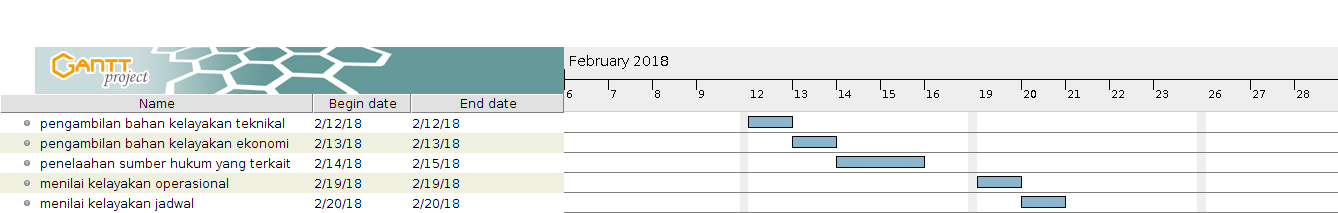
\includegraphics[width=1\textwidth]{./resources/gantt-jadwal-waktu}
  \caption{Jadwal Waktu Studi Kelayakan}
\end{figure}

\section{CAKUPAN KEGIATAN}

Cakupan kegiatan pada studi kelayakan ini hanya memerlukan pengumpulan beberapa fakta kelayakan apakah aplikasi yang dibangun ini dianggap perlu atau tidak, serta melihat terhadap produk hukum, apakah aplikasi ini bertentangan terhadap aturan tertentu atau tidak.

\section{TENAGA DAN BIAYA YANG DIPERLUKAN UNTUK STUDI KELAYAKAN}

Tenaga yang diperlukan untuk studi kelayakan ini hanya 1 (satu) orang fungsional Pranata Komputer sebagai pengolah data hasil pengumpulan fakta aturan aturan mengenai ketentuan umum dan tata cara perpajakan.

\end{document}